\documentclass{article}

% --- load packages ---
\usepackage[margin=1in]{geometry} % change the margins
\usepackage{amsmath} % useful math environments and commands like align
\usepackage[colorlinks,bookmarks,bookmarksnumbered,allcolors=blue]{hyperref} % hyperlinks between references
\usepackage{graphicx}  % include images
\usepackage[table,xcdraw]{xcolor}
\usepackage[caption=false]{subfig} % subfigures.  false option prevents conflicts in caption styling with other packages
\usepackage{booktabs} % better tables
\usepackage[capitalise]{cleveref} % better referencing. uses cref.
\usepackage[section]{placeins} % sometimes useful to prevent figures from floating out of a section
\usepackage{cite} % handles multiple citations in one command better
\usepackage{doi} % allow correct hypderlinking of DOIs
\usepackage[normalem]{ulem}
\usepackage{float}
\usepackage{minted}
\usepackage{pdfpages}
\usepackage{tikz}
\usepackage{csvsimple}
\usepackage{adjustbox, lipsum}
\usepackage{setspace}
\usetikzlibrary{tikzmark}

\useunder{\uline}{\ul}{}
\newcommand{\wide}{0.7\linewidth}


\begin{document}
\singlespacing
\title{}
\author{Landon Wright}
% put in \date{} if you don't want a date to appear, or enter a specific date, otherwise default is today's date.
\maketitle
% \begin{table}[H]
% 	\caption{Quasi-Newton progression}
% 	\centering
% 	\noindent\adjustbox{max width=\textwidth}{%
% \begin{tabular}{|r|c|c|c|c|c|}
% 	\hline
%   % \noindent\adjustbox{max width=\textwidth}{%
%   &\bfseries Start-value & \bfseries Value & \bfseries Step-direction & \bfseries Step-len & \bfseries Function-calls
%
%   \csvreader[head to column names]{output3.csv}{}%
%   {\\\thecsvrow & (\a, \b, \c)& \d & (\e, \f, \g) & \h & \i}
%   \\\hline
% \end{tabular}}
% \end{table}

\section{Matlab Code}

\subsection{Fminun Routine}
% \inputminted[xleftmargin=10pt,linenos]{matlab}{fminun.m}
\subsection{Driver}
% \inputminted[xleftmargin=10pt,linenos]{matlab}{fminunDriv.m}

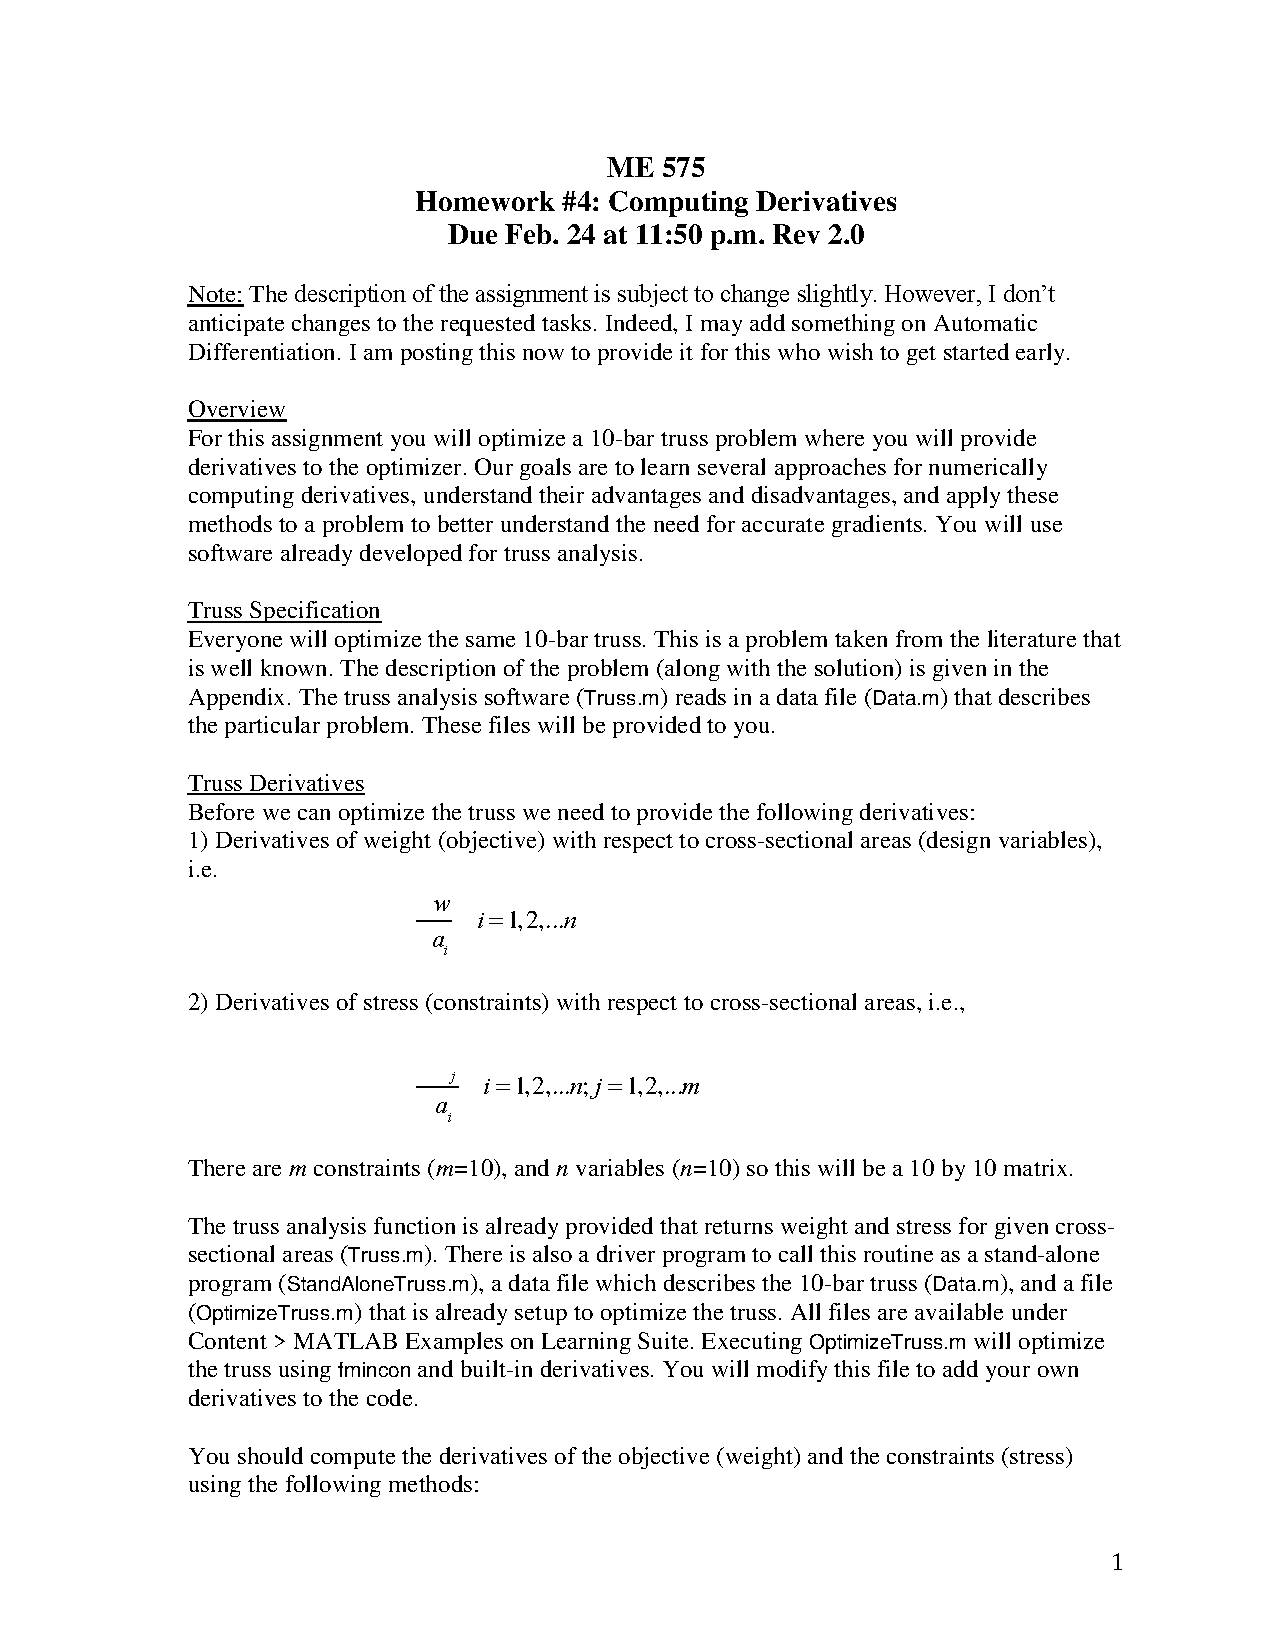
\includepdf[pages=-, pagecommand={}]{HW4.pdf}
\end{document}
